\documentclass{article}
\usepackage{tikz}
\usetikzlibrary{shapes,arrows,positioning,calc}

\begin{document}

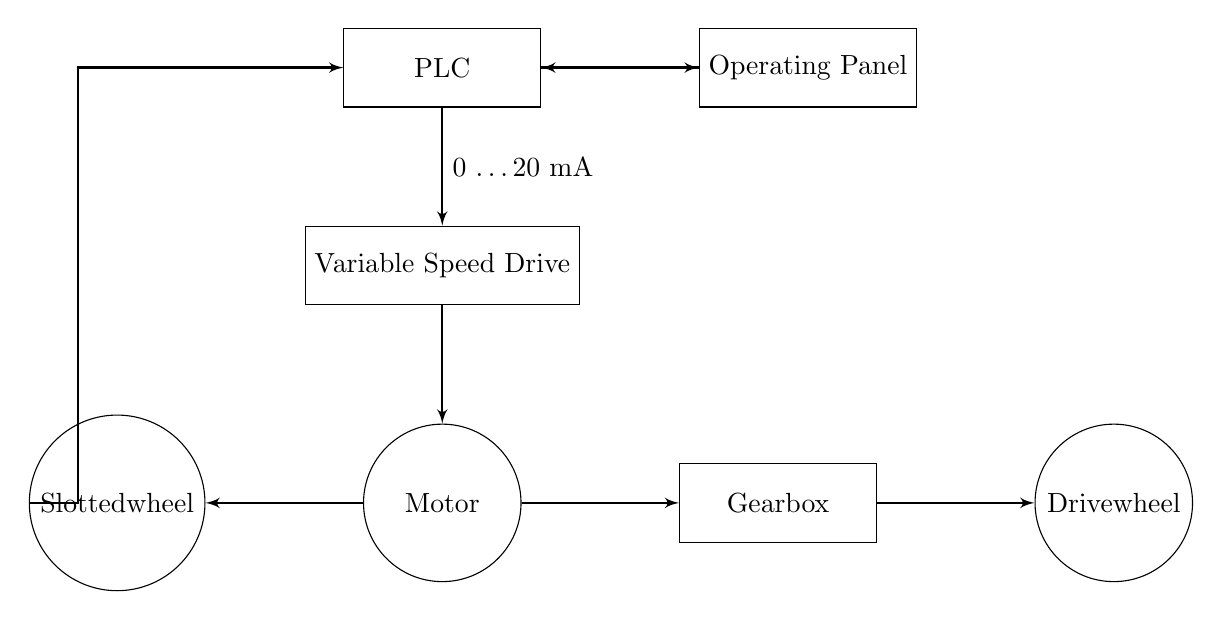
\begin{tikzpicture}[
    % Define styles for different types of blocks
    block/.style={
        rectangle,
        draw,
        text centered,
        minimum height=1cm,
        minimum width=2.5cm
    },
    circle_block/.style={
        circle,
        draw,
        text centered,
        minimum size=2cm
    },
    line/.style={
        draw,
        -latex',
        thick
    }
]

% Place the blocks
\node[block] (plc) {PLC};
\node[block, right=2cm of plc] (panel) {Operating Panel};
\node[block, below=1.5cm of plc] (vsd) {Variable Speed Drive};
\node[circle_block, below=1.5cm of vsd] (motor) {Motor};
\node[circle_block, left=2cm of motor] (slotted) {Slotted\\wheel};
\node[block, right=2cm of motor] (gearbox) {Gearbox};
\node[circle_block, right=2cm of gearbox] (drive) {Drive\\wheel};

% Draw the connections
% PLC to Operating Panel (bidirectional)
\draw[line] (plc) -- (panel);
\draw[line] (panel) -- (plc);

% PLC to VSD
\draw[line] (plc) -- node[right] {0 \ldots 20 mA} (vsd);

% VSD to Motor
\draw[line] (vsd) -- (motor);

% Motor connections
\draw[line] (motor) -- (slotted);
\draw[line] (motor) -- (gearbox);
\draw[line] (gearbox) -- (drive);

% Feedback loop from Slotted wheel to PLC
\draw[line] (slotted) -| ($(slotted) + (-0.5,0)$) |- (plc);

\end{tikzpicture}

\end{document}